\subsection{Pure \ch{NO} measurements with synthetic air}
\label{sec:no}

After confirming that our generator produced a clean Ozone stream, we
turned towards the question whether it is possible to actually measure
\ch{NO} or not. Furthermore we wanted to reach an experimental
estimate for the necessary reaction pathlength as computed in
Section~\ref{sec:requirements}.

\subsubsection{Setup}
\label{sec:no-setup}

To be able to measure the Nitrogen Monoxide concentration directly
without additional corrections and computations, we had to make sure
that the used sample air was Nitrogen Dioxide free. This lead us to
the setup depicted in Figure~\ref{fig:no-setup}. We used synthetic air
and \ch{NO} calibration gas with a known \ch{NO} concentration ($c =
\SI{8.177}{ppm}$) together with a mass flow controller to generate
precisely controlled sample air. To minimize the influence on the
pressure inside the cavity, we decided to overflow the air input
instead of bypassing the cavity pump as is done during a Helium
calibration. Thus we set the synthetic air flow to $\Phi_{\text{air}}$
to \SI{3}{\liter\per\minute}. The cavity itself was in the standard
setup described in Section~\ref{sec:inclusion}, except for the
reaction pathlength whch was varied between \SI{5}{\meter},
\SI{10}{\meter} and \SI{15}{\meter}. For each of these lengths we
varied the \ch{NO} calibration gas flow between \num{0} and
\SI{0.03}{\liter\per\minute}. As zeror air we used ambient lab air
together with a zero air cartridge.

\begin{figure}[htbp]
  \centering
  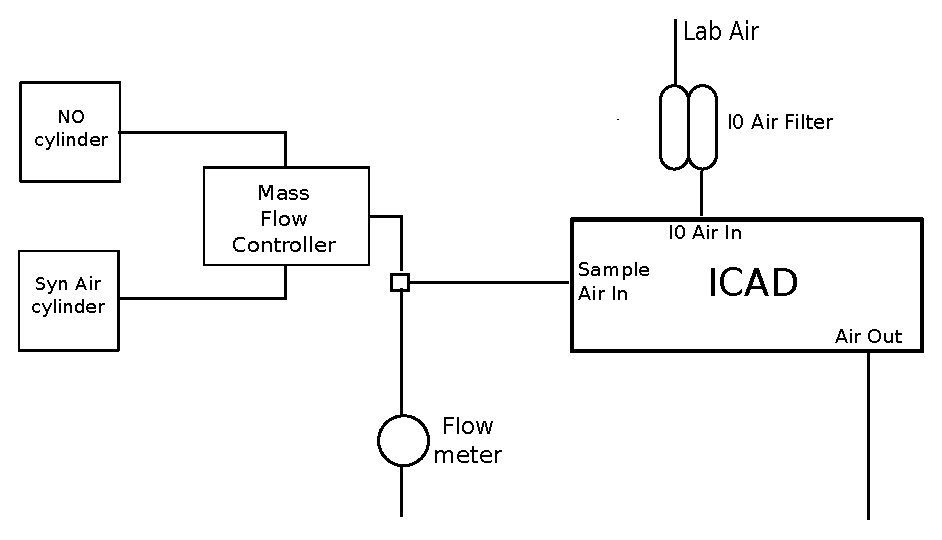
\includegraphics[width=0.6\textwidth]{no_setup.eps}
  \caption{Setup of the calibration measurement}
  \label{fig:no-setup}
\end{figure}

In order be able to compare the measured \ch{NO} concentration to the
actual concentration in the air stream, we had to convert the applied
\ch{NO} flow to a concentration, too. We were able to do this using the
following formula
\begin{align}
  c_{\ch{NO}} = c \cdot \frac{\Phi_{\ch{NO}}}{\Phi_{\text{air}} +
  \Phi_{\ch{NO}}}. \label{eq:c-flow}
\end{align}

\subsubsection{Results}
\label{sec:no-results}

Figure~\ref{fig:ts} shows the time series of the \ch{NO} and \ch{O3}
concentration. Each of the three clusters corresponds from left to
right to the reaction path length of \num{5}, \num{10} and
\SI{15}{\meter}. Turning first towards the Ozone concentration on the
right hand side, we see that its concentration is constant within its
error margins. These, however, are large. This is to be expected, as
the absorption cross section of \ch{O3} in the visual spectrum is weak
compared to the cross section of \ch{NO2} and has almost no
differential structure. If now the \ch{NO2} signal
becomes strong the fitting of the weaker \ch{O3} absorption becomes
harder and leads to larger errors. Nevertheless, the Ozone level seems
acceptably stable, which indicates that not to many Ozone destroying
reactions took place. This is again what we expected in this very pure
sample air which should only allow for the oxidation of
\ch{NO}. Lastly the shape of the Ozone time series does not seem to
depend on the reaction pathlength.

Looking at the \ch{NO} time series on the right hand side of
Figure~\ref{fig:ts} we see that the overall shape of the three
measurements are similar. For the reaction pathlength of $l=
\SI{5}{\meter}$ we see slight deviations. The rising flanks take
longer to reach a stable plateau than during the other two
measurements. Furthermore the first three plateaus are not visible,
however, the reason for this lies in the fact that they were
skipped during the measurement procedure. This behaviour cannot simply
be explained by a too short reaction path. If this were the case, the
depcited equilibria should all just lay lower, as the reaction dynamic
equilibrium would set for a lower, but \emph{constant} \ch{NO2}
concentration. Interstingly on the falling flanks the equilibria are
reached instantaneously (the small drop at \SI{50}{ppb} being a human
error). One possible explanation might lie in the adsorption behaviour
of teflon. For example if the Ozone were to be adsorbed to the tube
walls, this could lead to an effective increase in Ozone
concentration, accelerating the reaction and thus compensating the too
short pathlength. If, additionally, the adsorption time scale were in
the order of magnitude of our dwell time per flow, this could explain
why we have slowly increasing flanks, while the falling flanks
stabilize quickly. In the first case the adsorbed Ozone would have to
build up, because of the increased concentration, in the second case
there would alreade be enough Ozone adsorbed. The testing of this idea
was sadly outside the scope of this thesis, such that for the
following measurements we accepted this oddity and decided to work
with longer pathlengths (i.\,e.~$l = \SI{10}{\meter}$) which seem to
not express this behaviour.

\begin{figure}[htbp]
  \centering
  \input{images/20160222_NO_fixI0_NO_ts}
  \hfill
  \input{images/20160222_NO_fixI0_O3_ts}
  \caption{Timeseries of the \ch{NO} and \ch{O3} concentration. The
    three clusters correspond to the three used reaction pathlengths
    $l = 5, 10$ and \SI{15}{\meter}.}
  \label{fig:ts}
\end{figure}
\begin{figure}[H]
  \centering
  % GNUPLOT: LaTeX picture with Postscript
\begingroup
  \makeatletter
  \providecommand\color[2][]{%
    \GenericError{(gnuplot) \space\space\space\@spaces}{%
      Package color not loaded in conjunction with
      terminal option `colourtext'%
    }{See the gnuplot documentation for explanation.%
    }{Either use 'blacktext' in gnuplot or load the package
      color.sty in LaTeX.}%
    \renewcommand\color[2][]{}%
  }%
  \providecommand\includegraphics[2][]{%
    \GenericError{(gnuplot) \space\space\space\@spaces}{%
      Package graphicx or graphics not loaded%
    }{See the gnuplot documentation for explanation.%
    }{The gnuplot epslatex terminal needs graphicx.sty or graphics.sty.}%
    \renewcommand\includegraphics[2][]{}%
  }%
  \providecommand\rotatebox[2]{#2}%
  \@ifundefined{ifGPcolor}{%
    \newif\ifGPcolor
    \GPcolorfalse
  }{}%
  \@ifundefined{ifGPblacktext}{%
    \newif\ifGPblacktext
    \GPblacktexttrue
  }{}%
  % define a \g@addto@macro without @ in the name:
  \let\gplgaddtomacro\g@addto@macro
  % define empty templates for all commands taking text:
  \gdef\gplbacktext{}%
  \gdef\gplfronttext{}%
  \makeatother
  \ifGPblacktext
    % no textcolor at all
    \def\colorrgb#1{}%
    \def\colorgray#1{}%
  \else
    % gray or color?
    \ifGPcolor
      \def\colorrgb#1{\color[rgb]{#1}}%
      \def\colorgray#1{\color[gray]{#1}}%
      \expandafter\def\csname LTw\endcsname{\color{white}}%
      \expandafter\def\csname LTb\endcsname{\color{black}}%
      \expandafter\def\csname LTa\endcsname{\color{black}}%
      \expandafter\def\csname LT0\endcsname{\color[rgb]{1,0,0}}%
      \expandafter\def\csname LT1\endcsname{\color[rgb]{0,1,0}}%
      \expandafter\def\csname LT2\endcsname{\color[rgb]{0,0,1}}%
      \expandafter\def\csname LT3\endcsname{\color[rgb]{1,0,1}}%
      \expandafter\def\csname LT4\endcsname{\color[rgb]{0,1,1}}%
      \expandafter\def\csname LT5\endcsname{\color[rgb]{1,1,0}}%
      \expandafter\def\csname LT6\endcsname{\color[rgb]{0,0,0}}%
      \expandafter\def\csname LT7\endcsname{\color[rgb]{1,0.3,0}}%
      \expandafter\def\csname LT8\endcsname{\color[rgb]{0.5,0.5,0.5}}%
    \else
      % gray
      \def\colorrgb#1{\color{black}}%
      \def\colorgray#1{\color[gray]{#1}}%
      \expandafter\def\csname LTw\endcsname{\color{white}}%
      \expandafter\def\csname LTb\endcsname{\color{black}}%
      \expandafter\def\csname LTa\endcsname{\color{black}}%
      \expandafter\def\csname LT0\endcsname{\color{black}}%
      \expandafter\def\csname LT1\endcsname{\color{black}}%
      \expandafter\def\csname LT2\endcsname{\color{black}}%
      \expandafter\def\csname LT3\endcsname{\color{black}}%
      \expandafter\def\csname LT4\endcsname{\color{black}}%
      \expandafter\def\csname LT5\endcsname{\color{black}}%
      \expandafter\def\csname LT6\endcsname{\color{black}}%
      \expandafter\def\csname LT7\endcsname{\color{black}}%
      \expandafter\def\csname LT8\endcsname{\color{black}}%
    \fi
  \fi
    \setlength{\unitlength}{0.0500bp}%
    \ifx\gptboxheight\undefined%
      \newlength{\gptboxheight}%
      \newlength{\gptboxwidth}%
      \newsavebox{\gptboxtext}%
    \fi%
    \setlength{\fboxrule}{0.5pt}%
    \setlength{\fboxsep}{1pt}%
\begin{picture}(7776.00,4320.00)%
    \gplgaddtomacro\gplbacktext{%
      \csname LTb\endcsname%
      \put(682,704){\makebox(0,0)[r]{\strut{}$0$}}%
      \put(682,1123){\makebox(0,0)[r]{\strut{}$10$}}%
      \put(682,1542){\makebox(0,0)[r]{\strut{}$20$}}%
      \put(682,1961){\makebox(0,0)[r]{\strut{}$30$}}%
      \put(682,2380){\makebox(0,0)[r]{\strut{}$40$}}%
      \put(682,2798){\makebox(0,0)[r]{\strut{}$50$}}%
      \put(682,3217){\makebox(0,0)[r]{\strut{}$60$}}%
      \put(682,3636){\makebox(0,0)[r]{\strut{}$70$}}%
      \put(682,4055){\makebox(0,0)[r]{\strut{}$80$}}%
      \put(814,484){\makebox(0,0){\strut{}$4$}}%
      \put(1635,484){\makebox(0,0){\strut{}$6$}}%
      \put(2455,484){\makebox(0,0){\strut{}$8$}}%
      \put(3276,484){\makebox(0,0){\strut{}$10$}}%
      \put(4097,484){\makebox(0,0){\strut{}$12$}}%
      \put(4917,484){\makebox(0,0){\strut{}$14$}}%
      \put(5738,484){\makebox(0,0){\strut{}$16$}}%
      \put(6558,484){\makebox(0,0){\strut{}$18$}}%
      \put(7379,484){\makebox(0,0){\strut{}$20$}}%
    }%
    \gplgaddtomacro\gplfronttext{%
      \csname LTb\endcsname%
      \put(176,2379){\rotatebox{-270}{\makebox(0,0){\strut{}Concentration [ppb]}}}%
      \put(4096,154){\makebox(0,0){\strut{}Length [m]}}%
      \csname LTb\endcsname%
      \put(6392,3882){\makebox(0,0)[r]{\strut{}0.01\ \si{\liter\per\minute}}}%
      \csname LTb\endcsname%
      \put(6392,3662){\makebox(0,0)[r]{\strut{}0.03\ \si{\liter\per\minute}}}%
      \csname LTb\endcsname%
      \put(6392,3442){\makebox(0,0)[r]{\strut{}0.05\ \si{\liter\per\minute}}}%
      \csname LTb\endcsname%
      \put(6392,3222){\makebox(0,0)[r]{\strut{}0.1\ \si{\liter\per\minute}}}%
      \csname LTb\endcsname%
      \put(6392,3002){\makebox(0,0)[r]{\strut{}0.2\ \si{\liter\per\minute}}}%
      \csname LTb\endcsname%
      \put(6392,2782){\makebox(0,0)[r]{\strut{}0.3\ \si{\liter\per\minute}}}%
    }%
    \gplbacktext
    \put(0,0){\includegraphics{../images/20160222_NO_fixI0_NO_length}}%
    \gplfronttext
  \end{picture}%
\endgroup

  \caption{\ch{NO} concentration dependence on reaction path
    length. The data points are colored depending on the applied
    \ch{NO} flow. All data points were linearly interpolated. The
    results can also be found in the plot.}
  \label{fig:no-length}
\end{figure}

Comparing next the \ch{NO2} plateaus between multiple pathlengths, we
see that the concentrations seem to coincide. Averaging them and
plotting them over the pathlength we yield Figure~\ref{fig:no-length},
which confirms this assertion. The data points at coresponding flows
were linearly interpolated to make drifts more tangible. The fits are
also plotted in the figure. The interpolation showed that the slope
was undiscernible from zero in each case. At the \SI{5}{\meter}
setting one of the red and one of the violet data points seem to be
off. These two data points correspond to the rising flanks discussed
extensively above. It seems that at these two data points the
equilibrium had not been reached and we averaged too early.

\begin{figure}[htbp]
  \centering
  \input{images/20160222_NO_fixI0}
  \caption{Correlation plot of the computed and the measured \ch{pNO}
    concentration.}
  \label{fig:no-calib}
\end{figure}

Since Figure~\ref{fig:no-length} indicated that the measured
concentrations aret pathlength independent (except for the two outliers),
we can use all of them to research the correlation between our
measured concentrations and the ones computed from the flow by
Equation~\eqref{eq:c-flow}. The result can be seen in
Figure~\ref{fig:no-calib} together with a linear regression. The
regression formula yields

\begin{align*}
  y = \num{0.994 \pm 0.002}  \cdot x -\num{0.002 \pm 0.058}.
\end{align*}

Thus we see that the deviation between the measured and computed
concentration lies in the per mill regime. We see that under these
controlled conditions our converter works and does not introduce
tangible systematic errors. Figure~\ref{fig:ts} implies that a
\SI{10}{\meter} reaction path is sufficient and will therefore used
for the following experiments.

%%% Local Variables:
%%% mode: latex
%%% TeX-master: "../Bachelor"
%%% End:
